%% tags: [bellman-ford]
%% source: 2023-sp-redemption_midterm_02
\begin{prob}
    Suppose the Bellman-Ford algorithm with early stopping is run on the
    weighted graph shown below using node $s$ as the source (the edge weights are
    intentionally not shown). In the worst case, how many iterations of Bellman-Ford will
    be performed? That is, how many iterations of the outer \mintinline{python}{for}-loop will
    occur?

    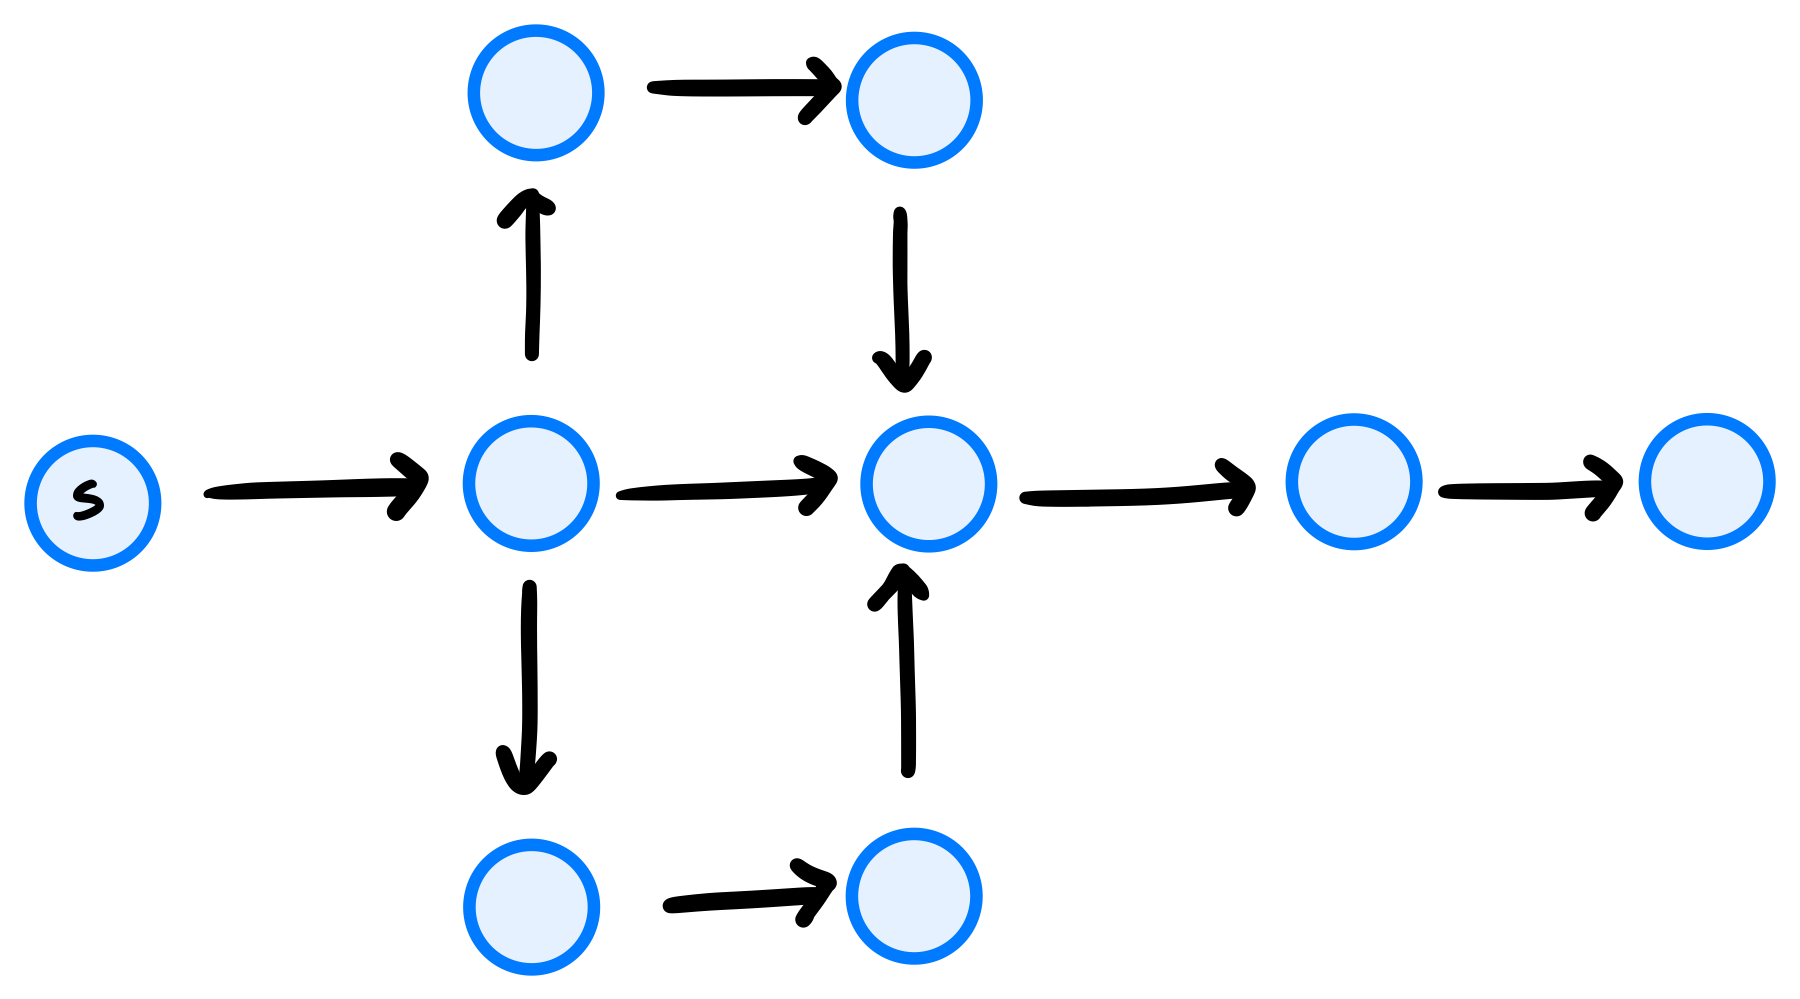
\includegraphics[width=.6\textwidth]{./g6.png}

    \begin{soln}
        7
    \end{soln}

\end{prob}
